
\subsubsection{補正手法の設計}

PDRによる位置推定の精度を向上させるため,本ライブラリは複数の補正手法を
組み合わせた設計を採用している.
これらの補正手法を統合的に扱うために,TrajectoryCorrectrorクラスを中心とした設計を提供している.
図\ref{fig:corrector-class}に示すように,補正処理はTrajectoryCorrector,
DriftCorrector,MapMatchCorrector,WirelessSignalCorrectorの4つの主要なクラスから構成されており,
それぞれが特定の補正機能を担当している.各補正クラスは独立して実装されており,
TrajectoryCorrectorを介して緩やかに結合され,保守性と拡張性を実現している.

\begin{figure}[H]
    \centering
    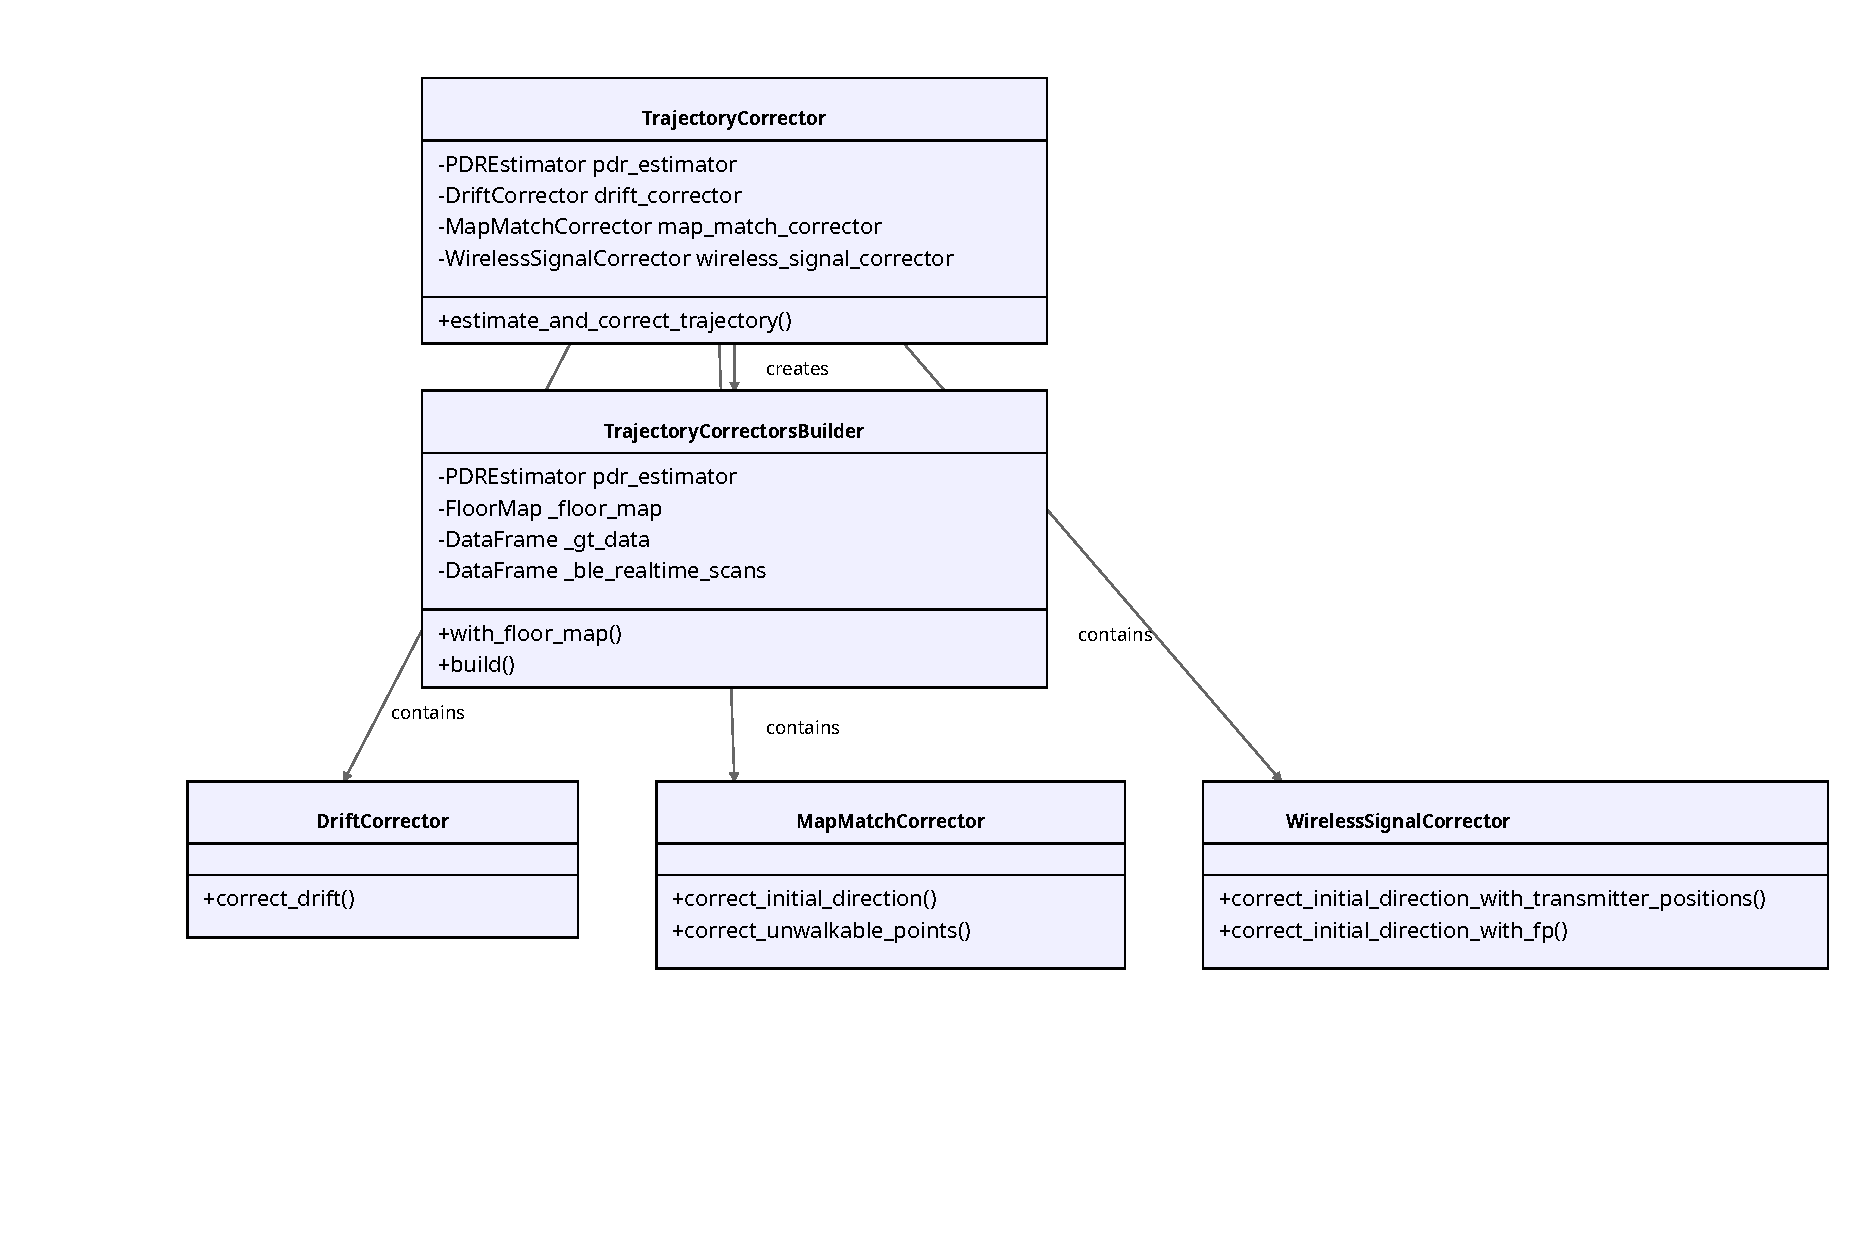
\includegraphics[width=\linewidth]{../image/trajectory_corrector.pdf}
    \caption{補正における主要クラス設計}
    \label{fig:corrector-class}
\end{figure}
% TODO:3.図の文字が小さくて読めない,図を大きくするといいかも

補正処理の柔軟な設定を可能にするため,TrajectoryCorrectorクラスは
Builderパターンを採用している.
これにより,複雑な補正処理を直感的なインターフェースで設定できる.
利用者はwith\_floor\_map()やwith\_wireless\_signal()などのメソッドチェーンを使用して
利用可能な環境情報に応じて必要な補正手法を選択的に組み合わせられる.
Listing\ref{lst:trajectory-corrector}にその例を示す.
例のようにフロアマップのみが利用可能な環境では,MapMatchCorrectorによる補正のみを
指定し,BLEビーコンも利用可能な環境では両方の補正を組み合わせて使用できる.
また各補正クラスは単体でも使用可能であり,特定の補正処理
のみを実行したい場合は,直接該当するクラスを利用を利用できる.


% TODO: PDFに謎のBLEの文字がある
\begin{lstlisting}[caption={TrajectoryCorrectorの使用例},label=lst:trajectory-corrector,float=h]
# フロアマップのみを使用する場合
corrector = TrajectoryCorrector.builder(pdr_estimator)
    .with_floor_map(floor_map)
    .build()

# フロアマップとBLE ビーコンを組み合わせる場合
corrector = TrajectoryCorrector.builder(pdr_estimator)
    .with_floor_map(floor_map)
    .with_wireless_signal(ble_scans beacon_positions)
    .build()
\end{lstlisting}

この設計の特徴は,新たな補正手法の追加が容易である点にある.例えば,
磁気フィンガープリントを用いた補正手法を追加する場合,MagneticCorrector
クラスを新規作成し,TrajectoryCorrectorsBuilderに対応するメソッドを
追加するだけで良い.この際,既存の補正クラスのコードを変更する必要が
ないため,システムの安定性を保ちながら機能を拡張するできる.
また,各補正手法は独立して実装されているため,個々の手法の改良や
バグ修正も他の機能に影響を与えず実装できる.

図\ref{fig:corrector-sequence}は,これらの補正処理の連携を示している.
TrajectoryCorrectorsBuilderを通じて必要な補正手法を指定し,buildメソッド
によってTrajectoryCorrectorのインスタンスを生成する.その後,
estimate\_and\_correct\_trajectoryメソッドを呼び出すと,指定された
補正手法が順次適用され,最終的な補正軌跡が得られる.この処理フローにより,
複数の補正手法を組み合わせた高度な位置推定が可能となっている.


\begin{figure}[H]
    \centering
    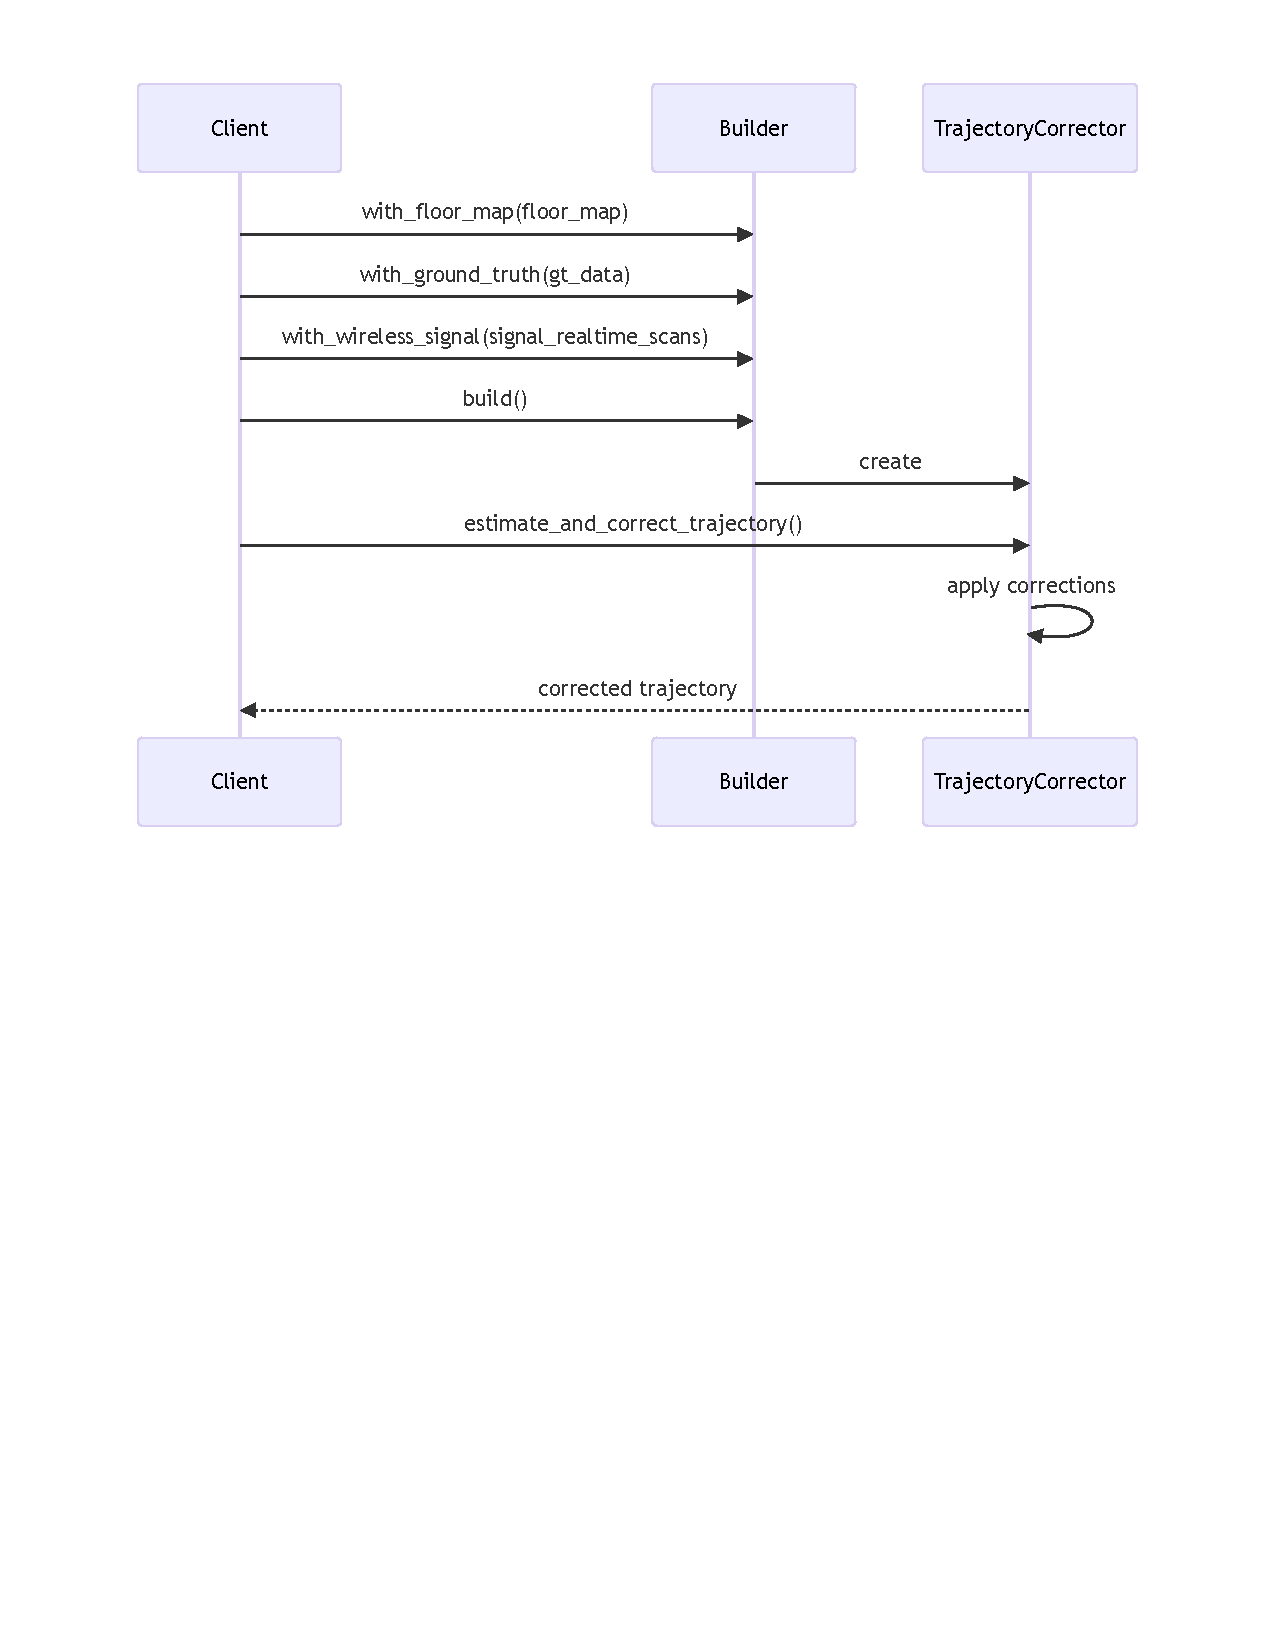
\includegraphics[width=\linewidth]{../image/corrector-flow-diagram.pdf}
    \caption{補正の処理フロー}
    \label{fig:corrector-sequence}
\end{figure}
